\documentclass[11pt,a4paper,bibtotocnumbered]{scrreprt}		                                   

\usepackage{graphicx}
\usepackage[dvipsnames]{xcolor}
\usepackage{a4}
\usepackage[onehalfspacing]{setspace}
\usepackage[ngerman]{babel}
\usepackage[utf8]{inputenc}
\usepackage{amsmath}
\usepackage{caption}
\usepackage{tabularx}
\usepackage{float}
\usepackage{listings}
\usepackage[babel,german=quotes]{csquotes}
\usepackage[printonlyused]{acronym}
\usepackage[linktoc=all, hidelinks]{hyperref}

\renewcaptionname{ngerman}\figureautorefname{Abb.}

\captionsetup[table]{belowskip=8pt}


\newcommand{\thema}{Eine domänenspezifische Sprache für die dialogische Logik}
\newcommand{\abgabedatum}{24.07.2015}
\newcommand{\zusammenfassung}{Vor dem Hintergrund einer sich wandelnden Welt versucht das Projekt \textit{Logic} den Bürger wieder stärker in den Mittelpunkt der Entscheidungsfindung zu rücken. Bedingt durch den Trend der Urbanisierung und Unterstützt von den Entwicklungen im Bereich der Smart City wächst der Bedarf an einfachen und durch neue Technologien unterstütze Methoden der Beteiligung. Hierzu wird eine domänenspezifische Sprache entwickelt, die in Verbindung mit der dialogischen Logik eine direkte und demokratisch faire Beteiligung auf Augenhöhe ermöglicht.}


\begin{document}



% ============================ FRONT MATTER
\pagenumbering{roman}
\begin{singlespace}
\begin{titlepage}

\vspace*{-3.5cm}

\begin{flushleft}
\hspace*{-1cm} 
\includegraphics[width=15.7cm]{htwg-logo}
\end{flushleft}

\vspace{2.5cm}

\begin{center}
	\huge{
		\textbf{\thema} \\[5cm]
	}
	\Large{
		\textbf{Tobias Keh, Simon Kessler}} \\[6.5cm]
	\large{
		\textbf{Konstanz, \abgabedatum} \\[2.3cm]
	}
	
	\Huge{
		\textbf{{\sf SEMINARARBEIT}}
	}
\end{center}

\end{titlepage}
\setcounter{page}{1}
\begin{center}
{\Large \textbf{Zusammenfassung (Abstract)}}
\end{center}

\bigskip

\begin{center}
	\begin{tabular}{p{2.8cm}p{10cm}}
		Thema: & \thema \\
		 & \\
		Abgabedatum: & \abgabedatum \\
		 & \\
	\end{tabular}
\end{center}

\bigskip

\noindent
\zusammenfassung
\end{singlespace}


\tableofcontents
\listoffigures
\listoftables

\chapter*{Abkürzungsverzeichnis} 

% Alphabetisch sortieren
\begin{acronym}[LAENGE]
\acro{DSL}{domänenspezifische Sprache}
\acro{EBNF}{Erweiterte Backus-Naur-Form}
\end{acronym}

\cleardoublepage
% ============================ ENDE FRONT MATTER



% ============================ HAUPTTEIL THESIS
\pagenumbering{arabic}


% ============================ CHAPTER
\chapter{Einleitung und Motivation} % Simon

Die Demokratie wandelt sich und versucht sich neu zu erfinden. 
Konzepte wie die \emph{deliberative Demokratie} erhalten unter dem Schlagwort \emph{Demokratie 2.0} neuen Zulauf. 
Auch die zunehmende Vernetzung der Gesellschaft durch das Internet trägt zu diesem Trend bei. 
Während in einer nicht vernetzten Welt Bürger nur sehr wenige Berührungs- und Einflusspunkte mit der Politik haben (z. B. während den Wahlen), kann das Internet helfen, Bürger aktiv in die politische und demokratische Entscheidungsfindung miteinzubeziehen.
Eng mit \emph{Liquid Democracy} verwandt, ermöglicht dieser Ansatz es den Bürgern, für einzelne Gesetze abzustimmen und Argumente einzubringen bzw. Diskussionen zu führen.
Die Diskussionen folgen bisher einem unstrukturierten Ablauf von Argumenten.
Hier könnte die \emph{dialogische Logik} zu einem geordneten, gesteuerten und fairen Dialog verhelfen.

Die Regeln der dialogischen Logik und ihre formale Darstellung sind zwar klar und deutlich, verhindern jedoch den Zugang der breiten Masse zu diesem Werkzeug.
Oder wie Ludwig Wittgenstein einst formulierte:
\begin{quote}
\enquote{Die Grenzen meiner Sprache bedeuten die Grenzen meiner Welt.}
\end{quote}
Das heißt, wollen wir wirklich Bürger einer Demokratie 2.0 ausgrenzen, die diese neue und innovative Form des Dialogs nicht beherrschen? Oder wollen wir Wege finden, auch diesen Menschen den dialogischen Dialog zu ermöglichen?

In dieser Projektarbeit soll deshalb eine \ac{DSL} entwickelt werden, die es ermöglicht einen dialogischen Dialog mit annähernd natürlichsprachlichen Elementen zu formulieren. 
Dabei liegt der Fokus auf einer einfachen Erlernbarkeit der Sprache.

Die Arbeit gliedert sich in eine weitere Motivation für die Arbeit, Erläuterung der theoretischen Grundlagen, Definition der Syntax, Evaluierung von Anwendungsfällen und einem abschließenden Fazit und Ausblick.
Es erfolgt eine Beschränkung auf die Syntax der Sprache, wobei anwendungsspezifische Beispiele für die semantische Auswertung genannt werden.

% ============================ CHAPTER
\chapter{Theoretische Grundlagen}  % Tobi
Inhalt dieses Kapitel sind die theoretischen Grundlagen des Projekts. Hierzu werden kurz die dialogische Logik, domänenspezifische Sprachen, Grammatiken und deren Einordnung in die Chomsky-Hierarchie und die Unterstützung durch Werkzeuge betrachtet.

\section{Dialogische Logik}
Die dialogische Logik wurde von Kuno Lorenz und Paul Lorenzen entwickelt. Sie stellt einen spieltheoretischen und semantiknahen Ansatz zur Logik dar. Dabei bildet sie, ganz im Sinne von Peter Wegners Leitgedanke \emph{"Why interaction is more powerful than algorithms"}, eine Erweiterung der formalen Logik durch die Orientierung am menschlichen Verhalten, beziehungsweise am menschlichen Dialog.
Im Gegensatz zur formalen Logik erlaubt die dialogische Logik den Dialog ohne dritte Partei in Form eines Schiedsrichters.

Aussagen der dialogischen Logik bestehen aus Elementaraussagen beziehungsweise aus Teilaussagen, die sich aus Elementaraussagen zusammensetzen. Aussagen werden unter Verwendung von Junktoren ($\land, \lor, \lnot, \to$) und Quantoren ($\exists, \forall$) formuliert.

Ein Regelwerk aus Rahmenregeln für den Dialog und Angriffs- beziehungsweise Abwehrregeln für die logischen Operatoren bilden die formale Grundlage der dialogischen Logik. Über diese werden der Ablauf des Dialogs und der Angriff beziehungsweise die Verteidigung von Elementar-, Teil- und vollständigen Aussagen genau geregelt.

\section{Domänenspezifische Sprachen}
Die Modellierung von Sachverhalten spielt sich immer in einer gewissen Fachdomäne ab. Um die Begrifflichkeiten und Eigenschaften einer solchen Domäne korrekt abbilden und einsetzen zu können, bietet sich die Verwendung einer domänenspezifischen Sprache an. Der Einsatz dieser Art von Sprachen in der Informatik bietet zum einen die Möglichkeit, dass Domänenexperten die Modellierung auch ohne Informatikkenntnisse durchführen können. Zum anderen wird der Sprachschatz genau auf den Umfang der jeweiligen Domäne begrenzt, was eine Beschränkung der mit der domänenspezifischen Sprache erstellten Modelle auf die jeweilige Domäne ermöglicht.
In der Informatik gibt es drei unterschiedliche Arten domänenspezifische Sprachen zu definieren.
\\
\\
1. Einschränkung einer vorhandenen allgemeinen Sprache
Bei dieser Art der Definition wird eine bereits vorhandene Sprache wie beispielsweise UML oder XML verwendet. Diese wird mit bestimmten Regeln soweit eingeschränkt, dass nur noch eine Benutzung im Sinne der entsprechenden Domäne möglich ist. Allerdings ist die Einschränkung mitunter kompliziert, da jede Möglichkeit der Sprache bedacht und entsprechend erlaubt oder unterbunden werden muss. Der bei allgemeinen Sprachen oft auftretende und durch die Beschränkung oftmals noch umfangreichere syntaktische Ballast ist dann ebenso Teil der definierten domänenspezifischen Sprache. Die Vorteile liegen hierbei darin, eine bereits vorhandene Sprache mit deren Tooling verwenden zu können. Die Nachteile überwiegen aber deutlich, da auf diese Art und Weise definierte domänenspezifische Sprachen sehr unflexibel sind und die Syntax vollständig von der eingeschränkten allgemeinen Sprache bestimmt wird.
\\
\\
2. Interne DSL
Hierbei wird eine vorhandene allgemeine Programmiersprache als Wirtssprache für die domänenspezifische Sprache genutzt. Die domänenspezifische Sprache wird hierbei als Fluent API programmatisch definiert. Obwohl die Modelle immer noch in der ursprünglichen Programmiersprache verfasst werden, entsteht durch diese Art der API eine auch für Laien gut verständliche Sprache. Zur Definition einer solchen API werden Methodenaufrufe wie folgt hintereinander gehängt:
\\
\\
\textit{Startsymbol.Methodenaufruf1.Methodenaufruf2.Methodenaufruf3}\\
oder\\
\textit{Elementaraussage(''Die Sonne scheint'').DarausFolgt(''Es ist heiß'').AussageEnde()}
\\
\\
Diese Aufrufkette ist auch für Laien verständlich und kann, je nach Umfang und Schwierigkeitsgrad der Sprache, auch von diesen erstellt werden. Die Vorteile liegen bei dieser Art der Definition darin, eine bereits vorhandene Sprache zu verwenden und auf deren Tooling zurückgreifen zu können. Des Weiteren ist der Wartungs- und Entwicklungsaufwand mittelmäßig bis gering. Von Nachteil ist, dass die Wirtssprache erlernt werden muss, beziehungsweise Fachwissen bei den Anwendern vorhanden sein muss. Ein weiterer Nachteil ist, dass die Aufrufketten der Fluent API zwar gut lesbar und verständlich sind, aber trotzdem noch weit entfernt von der Flexibilität und syntaktischen Prägnanz einer vollständig erstellten Sprache sind (Externe DSL).
\\
\\
3. Externe DSL
Die flexibelste und syntaktisch eleganteste Variante ist die Definition einer externen DSL. Hierbei werden konkrete und abstrakte Syntax meist in Form einer Grammatik vollständig entworfen. Dies bietet größtmögliche Freiheiten bei der Gestaltung der konkreten Syntax und somit eine bestmögliche Verständlichkeit und Anwendbarkeit durch den Benutzer einer bestimmten Domäne. Der Nachteil liegt hierbei im größeren Entwicklungs- und Wartungsaufwand. Jedoch ist dieser im Bereich der textuellen domänenspezifischen Sprachen mittlerweile durch die Verfügbarkeit von mächtigen Tools vertretbar.
Im Projekt \textit{Logic} kommt diese Art der DSL zum Einsatz, da hier die bestmögliche Benutzbarkeit wichtigstes Kriterium ist.

\section{Grammatiken} 
Da im Zuge des Projekts eine externe DSL definiert wird, müssen konkrete und abstrakte Syntax mittels einer Grammatik definiert werden. Besonders die konkrete Syntax ist hier von besonderer Wichtigkeit, da diese die Schnittstelle zum Benutzer darstellt und somit über die Akzeptanz und den Erfolg der domänenspezifischen Sprache entscheidet.
Grammatiken können mit Hilfe der Chomsky Hierarchie kategorisiert werden. Diese Hierarchie definiert vier Typen, welche sich durch den Umfang der durch die Grammatik erlaubten Produktionen unterscheiden.
\\
\\
Typ 3: Reguläre Grammatiken\\
Reguläre Ausdrücke mit genau einem Terminal auf der linken Seite und genau einem Terminal auf der rechten Seite beziehungsweise ein Terminal gefolgt von einem Nichtterminal, beispielsweise \textit{A: wB}
\\
\\
Typ 2: Kontextfreie Grammatiken\\
Produktionen mit genau einem Terminal auf linken Seite und Kombinationen aus Terminalen und Nichtterminalen auf der rechten Seite. \\Zum Beispiel: \textit{A: wB $\vert$ wBw $\vert$ wwBw}
\\
\\
Typ 1: Kontextsensitive Grammatiken\\
Kontextsensitive Grammatiken erweitern die Regeln der kontextfreien Grammatiken um die Möglichkeit, auf der linken Seite einer Produktion Kombinationen von Terminalen und Nichtterminalen anzugeben. Dadurch können einzelne Regeln abhängig von einem bestimmten Kontext aus Terminalen und Nichtterminalen sein. \\Beispielsweise: \textit{wAw: wB $\vert$ wBw $\vert$ wwBw}
\\
\\
Typ 0: Allgemeine Chomsky Grammatiken\\
Alle übrigen formalen Grammatiken sind vom Typ 0, der allgemeinen Chomsky Grammatiken.
\\
\\
Das initiale Vorhaben Chomskys war es eine formale Grammatik für natürliche Sprache zu definieren. Allerdings ist ihm dies nicht gelungen, da natürliche Sprache zu variabel und mehrdeutig ist und für Maschinen, ohne Informationen über den Kontext einer Aussage zu kennen, eventuell überhaupt nicht entscheidbar ist. Daher ist natürliche Sprache unterhalb von Typ 0, also außerhalb der Chomsky Hierarchie anzuordnen. Hierbei wird das Problem der maschinellen Anwendung der dialogischen Logik deutlich sichtbar. Allgemeine Programmiersprachen und externe DSLs, die auf die von uns eingesetzte Art definiert werden, besitzen Typ 2 Grammatiken.
Sprachen mit Grammatiken, die unterhalb des Typ 2 liegen, sind für Maschinen nur schwer zu verarbeiten, da der Parser, der die Produktionen verarbeitet, pro Verarbeitungsschritt zu viele mögliche Pfade hat und somit einen zu großen Aufwand betreiben muss, um eine Entscheidung für den aktuellen Input zu treffen. Dies kann sogar soweit gehen, dass eine Produktion nicht entscheidbar ist und der Parser nicht terminiert.
Aussagen für die Anwendung der dialogischen Logik in natürlicher Sprache folgen jedoch einer Grammatik, die außerhalb der Chomsky Hierarchie liegt. Um diese Lücke zu schließen, ist eine domänenspezifische Sprache notwendig, die eine Typ 2 Grammatik besitzt um maschinell verarbeitbar zu sein und die eine konkrete Syntax besitzt, die möglichst nah an natürlicher Sprache liegt.

\section{Werkzeugunterstützung}
Beim Entwurf einer externen DSL muss das Rad nicht neu erfunden werden, sondern es kann auf eine breite Palette an performanten Tools zurückgegriffen werden. Zur Definition der Grammatik kommt hierbei Xtext zum Einsatz. Bei Xtext handelt es sich um ein Open-Source Projekt aus dem Umfeld des Eclipse Modeling Frameworks zur Definition textueller DSLs.
Die Grammatik wird in einer leicht modifizierten Erweiterten Backus Naur Form (EBNF) angegeben. Hierbei wird die EBNF um Variablen erweitert, über die im späteren Verlauf der Tool Benutzung auf einzelne Inhalte des Modells zugegriffen werden kann. Xtext bietet eine automatische Generierung von Werkzeugen. Hierbei werden ein Parser für die domänenspezifische Sprache, ein EMF Metamodell zur Validierung von Modellen und ein Eclipse-basierter Texteditor generiert. Der Texteditor verfügt über Funktionen wie Syntax Highlighting, Code Completion und Fehlererkennung in Echtzeit.

% ============================ CHAPTER
\chapter{Die Sprache \enquote{Logic}} % Simon

In diesem Kapitel soll die entwickelte Sprache \enquote{Logic} mit ihrer Grammatik und Beispielen vorgestellt werden.
Ziel der Sprache ist es, eine Brücke zwischen der Semantik und der Syntax Ebene zur maschinellen Verarbeitung zu bilden (vgl. \cite[Folie 11]{OrtnerDL}).
Dabei soll das \enquote{Gemeinte} möglichst simpel in der formalen dialogischen Logik ausgedrückt werden können.

\section{Meta-Modell}

Die Sprache basiert auf einem Meta-Modell, welches es erlaubt, die einzelnen Elemente der Sprache maschinell in anderen Anwendungen zu verarbeiten.
In \autoref{metamodell} ist das verwendete Meta-Modell ersichtlich.

\begin{figure}[htbp]
\centering
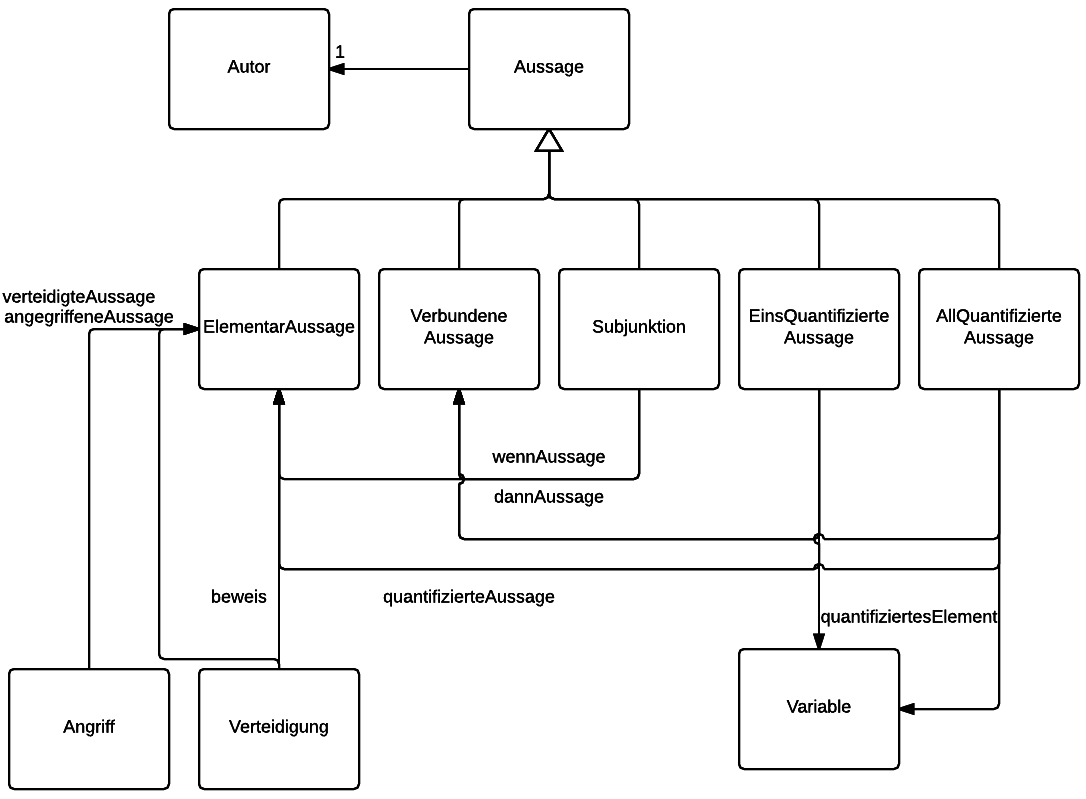
\includegraphics[width=1\textwidth]{img/metamodell.png}
\caption{Meta-Modell von \enquote{Logic}}
\label{metamodell}
\end{figure}

Jede Aussage besitzt exakt einen Autor, der namentlich genannt wird.
Dies ist wichtig, um im Dialog eine eindeutige Zuweisung von Aussagen vornehmen und entsprechend referenzieren zu können.
Eine Aussage wiederum ist im konkreten Fall ein Typ aus der Menge \{ElementarAussage, VerbundeneAussage, Subjunktion, EinsQuantifizierteAussage, AllQuantifizierteAussage\}. 
ElementarAussage besitzt ein Attribut mit dem Inhalt der Aussage als Textform.
Der Typ VerbundeneAussage besteht aus einer ElementarAussage und einer weiteren Aussage, verbunden durch ein Schlüsselwort (Adjunktor oder Konjunktor).
Auch die Quantifizierung von Aussagen wird unterstützt, da dies einige weitere Anwendungsfälle eröffnet.
Eine quantifizierte Aussage assoziiert eine Variable (Text), die entsprechend quantifiziert wird und eine Aussage, für welche die Variable gebunden wird.
Subjunktionen referenzieren eine ElementarAussage über das Attribut \enquote{wenn} und eine VerbundeneAussage oder ElemtarAussage über das Attribut \enquote{dann}.
Dies entspricht dem folgenden Schema: \enquote{wenn} $\rightarrow$ \enquote{dann}.
Auch die Angriffe und Verteidigungen im dialogischen Dialog finden sich im Meta-Modell wieder. 
Diese beziehen sich stets auf ein Objekt des Typs ElementarAussage.
Die Verteidigung referenziert dabei sowohl die verteidigte Aussage als auch eine Aussage, die als Beweis dient.

Um Formulierungen verständlich und nicht zu komplex werden zu lassen, wurden gewisse Einschränkungen vorgenommen. 
So können in einer Subjunktion keine weiteren Subjunktionen verschachtelt werden.
Eine Aussage wie z. B. \enquote{wenn $\rightarrow$ (wenn $\rightarrow$ dann)} ist somit ausgeschlossen.
Solche Konstrukte kommen in Dialogen aber recht selten vor und stellen nur eine unwesentliche Einschränkung dar.
Diese Einschränkungen fördern das einfache Verständnis von Dialogen und verhindern, dass kompliziert geschachtelte Formulierungen verwendet werden, die den Bürgern unter Umständen nicht verständlich sind.

Das Meta-Modell liegt als \emph{ecore} (vgl. \cite{Ecore}) Datei vor, welche interoperabel mit vielen Eclipse-Projekten ist. 
Da es sich um ein XML-Format handelt, ist auch eine anderweitige Verwendung mit geringem Aufwand möglich.
So wäre auch durchaus ein graphischer Editor basierend auf diesem Meta-Modell vorstellbar.
Hier sei insbesondere auf das Projekt \emph{Spray} (vgl. \cite{Spray}) verwiesen, an dem die HTWG (Prof. Dr. Marko Boger) beteiligt ist.

\section{Grammatik}

Unser Vorschlag für die konkrete Syntax, um das Meta-Modell abzubilden ist in \autoref{grammatik} ersichtlich.
Die Notation ist an die \ac{EBNF} angelehnt und beschreibt die Grammatik für das Tool Xtext \cite{Xtext}.
Der Quellcode zum Projekt kann bei GitHub gefunden werden \cite{GitHubCode}.

\begin{table}[htbp]
\centering
\caption{Wichtige Terminale der DSL}
\label{terminale}
\begin{tabularx}{\textwidth}{|p{3cm}|X|}
\hline
« 				& Öffnendes Symbol für eine Elementaraussage.  \\ \hline
» 				& Schließendes Symbol für eine Elementaraussage.  \\ \hline
und  			& Konjunktion zwischen zwei Aussagen.   \\  \hline
oder  		& Adjunktion zwischen zwei Aussagen.   \\  \hline
.     			& Schließt eine Aussage.   \\  \hline
:				& Schließt die Nennung des Autors.   \\  \hline
wenn, weil	& Öffnet in einer Subjunktion den \enquote{Wenn}-Teil.   \\  \hline
dann, folgt daraus	& Leitet in einer Subjunktion den \enquote{Wenn}-Teil ein.   \\  \hline
für mindestens einen, eine, ein & Einsquantifiziert eine Variable (Text).   \\  \hline
für alle & Allquantifiziert eine Variable (Text).   \\  \hline
gilt:				& Öffnet die Definition einer Aussage, auf die sich die quantifizierte Variable bezieht.   \\  \hline
Ich bezweifle:		& Eröffnet einen Angriff auf eine Elementaraussage.   \\  \hline
Ich beweise:		& Eröffnet eine Verteidigung einer Elementaraussagen.   \\  \hline
durch:		& Leitet die Nennung einer Elementar oder verbundenen Aussage ein, die als Beweis in einer Verteidigung dient.   \\  \hline
\end{tabularx}
\end{table}

\begin{figure}[htbp]
\centering
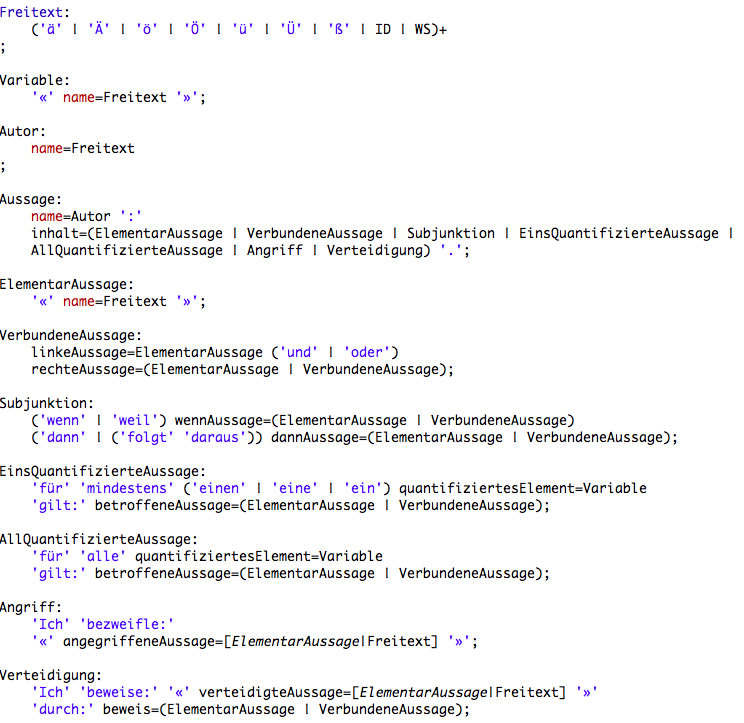
\includegraphics[width=1\textwidth]{img/grammatik.png}
\caption{Grammatik von \enquote{Logic}}
\label{grammatik}
\end{figure}

Wichtige Terminale sind in \autoref{terminale} ersichtlich.
Es wurden explizit Wörter und Zeichen gewählt die einerseits beim Lesen einer Aussage nicht stören und den natürlichsprachlichen Eindruck so wenig wie möglich beeinträchtigen. Andererseits aber auch eine klare Struktur bieten, um Aussagen auch ohne Tool-Unterstützung schnell erfassen bzw. formulieren zu können.

Da in der deutschen Sprache Guillemets («,») recht selten verwendet werden, trotzdem im Lesefluss kaum stören, bieten sich diese gut als \enquote{Klammer} für Aussagen an.
So können auch weiterhin normale Anführungszeichen in Aussagen vorkommen.
Durch die generischen Terminale für Subjunktionen, Quantoren, Angriffe und Verteidigungen ist sichergestellt, dass für eine Vielzahl von Aussagen ein annähernd korrekter deutscher Satz entsteht, der sich flüssig lesen lässt.


\section{Editor und Parser}

Der generierte Editor und Parser unterstützen Autovervollständigung von eingegebenem Text (vgl. \autoref{completion2}) bzw. von Schlüsselwörtern (vgl. \autoref{completion1}).
Falscheingaben werden sofort während des Tippens erkannt und rot unterstrichen, um den Anwender bei der Formulierung seiner Aussage zu unterstützen.
Eine weitere hilfreiche Funktion ist die Darstellung einer Baumansicht der Aussagen (vgl. \autoref{outline}).
Hierbei ist anzumerken, dass die Baumansicht noch nicht vollständig entwickelt ist.
Die ersichtlichen \enquote{$<$unnamed$>$} Knoten können mit angepassten Content-Providern noch mit sinnvollen Bezeichnern versehen werden.

\begin{figure}
\centering
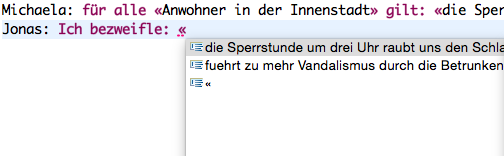
\includegraphics[width=0.5\textwidth]{img/completion2.png}
\caption{Autovervollständigung von Text}
\label{completion2}
\end{figure}

\begin{figure}
\centering
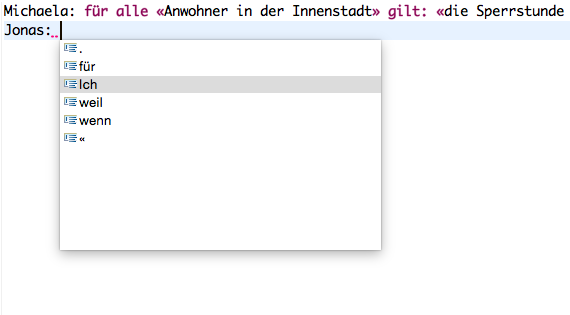
\includegraphics[width=0.5\textwidth]{img/completion1.png}
\caption{Autovervollständigung von Schlüsselwörtern}
\label{completion1}
\end{figure}

\begin{figure}
\centering
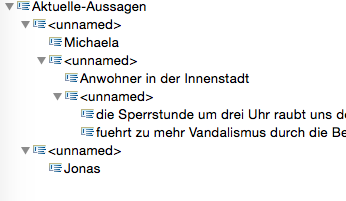
\includegraphics[width=0.5\textwidth]{img/outline.png}
\caption{Baumansicht der Aussage}
\label{outline}
\end{figure}

Der Editor wird als Eclipse-Plugin generiert und kann in anderen Eclipse RCP Anwendungen einfach integriert werden.
Es ist auch möglich, das durch das Parsen entstandene Modell einer Aussage in eine normalen Java-Anwendung zu laden \cite{XtextLoadJava}.
Sollte eine Eclipse-basierte Umgebung nicht möglich sein, so kann der Parser als Java-Applikation exportiert und in anderen Projekten als Backend genutzt werden.
In diesem Fall steht dann der Editor nicht zur Verfügung, könnte jedoch nachgebaut werden (z .B. für Internetprojekte).


\section{Beispiele}

Nachfolgend soll die Grammatik der Sprache mit Beispielen verdeutlicht werden.
Zuerst werden einfache logische Ausdrücke vorgestellt, die dann angegriffen bzw. verteidigt werden und abschließend in einem vollständigen Beispieldialog münden.

\subsection{Logische Aussage}

Eine einfache Aussage, wie z. B. \enquote{Die Politik hat versagt} (Max Muster) lassen sich mit der \ac{DSL} als \enquote{Max Muster: «Die Politik hat versagt».} ausdrücken.
Zusammengesetzte Aussagen werden wie folgt formuliert: \enquote{Max Muster: «Die Politk hat versagt» und «das Volk ist politikverdrossen».}.
Die Subjunktion könnte so verwendet werden: \enquote{Max Muster: weil «das Volk politikverdrossen ist» folgt daraus «dass die Politk versagt hat».}.
Quantifizierung von Variablen ist praktisch für verallgemeinernde Aussagen, wie \enquote{Max Muster: für alle «Jugendlichen» gilt: «dass sie nicht wissen, was sie einmal arbeiten möchten».}.

\subsection{Angriff und Verteidigung}

Insbesondere der strukturierte Ablauf von Diskussionen lässt sich mit der dialogischen Logik hervorragend unterstützen. Deshalb sollen nachfolgend ein Beispiel für einen Angriff bzw. eine Verteidigung folgen.
Beispiel Angriff: \enquote{Petra Maier: Ich bezweifle «das Volk politikverdrossen ist».}.
Eine Verteidigung könnte lauten: \enquote{Max Muster: Ich beweise «das Volk ist politikverdrossen» durch: «die Wahlbeteiligung sinkt seit den letzten zehn Jahren kontinuierlich».}.

\subsection{Gesamtdialog}

Nachfolgend wird eine Diskussion um die Sperrstunde in der Konstanzer Innenstadt mit Hilfe der dialogischen Logik und der \ac{DSL} \enquote{Logic} geführt. 
Alle Namen und Argumente sind rein fiktiv.

Michaela P. (Anwohnerin): für alle «Anwohner in der Innenstadt» gilt: «die Sperrstunde um 3 Uhr raubt uns den Schlaf» und «führt zu mehr Vandalismus durch die Betrunkenen».\\
Jonas F. (Student): Ich bezweifle «führt zu mehr Vandalismus durch die Betrunkenen».\\
Michaela P. (Anwohnerin): Ich beweise «führt zu mehr Vandalismus durch die Betrunkenen» durch: «die Polizeistatistik von 2014, die einen klaren Zusammenhang herstellt». \\
Jonas F. (Student): Ich bezweifle: «die Sperrstunde um 3 Uhr raubt uns den Schlaf».\\
Michaela P. (Anwohnerin): Ich beweise: «die Sperrstunde um 3 Uhr raubt uns den Schlaf» durch: «eine Unterschriftenliste aller Anwohner, die belegt, dass sie sich gestört fühlen».

% ============================ CHAPTER
\chapter{Anwendungsfälle} % Simon

Um bewerten zu können, ob die entworfene Sprache eine Bereicherung für vorhandene Probleme bzw. Anwendungen darstellt, sollen in diesem Kapitel einige Anwendungsfälle evaluiert werden.

\section{Syntax und Semantik} % Tobi
Bei der Definition domänenspezifischer Sprachen können zum einen konkrete und abstrakte Syntax und zum anderen statische und dynamische Semantik definiert werden.
Während die Definition der Syntax zwingend erforderlich ist, so ist die Semantik abhängig vom konkreten Einsatzzweck der Sprache. Mit statischer und dynamischer Semantik wird festgelegt, was aus Modellen der Sprache tatsächlich entstehen soll. Hierbei handelt es sich um eine Vielzahl an Möglichkeiten, wie beispielsweise Dokumentation, Programmcode, HTML Code für eine Webseite, oder aber auch Maschinencode zum Ausführen auf einem Computer. Entsprechende Einsatzszenarien für das \textit{Logic} Projekt werden in einem späteren Kapitel genannt.
Auch für die Semantik gibt es entsprechende Tool Unterstützung. Hierbei kommt das Xtend Projekt zum Einsatz, das mit dem Xtext Projekt in Beziehung steht. Dieses Tool ermöglicht Model-to-Model Transformationen, um Modelle in eine andere Form zu überführen, wie beispielsweise bei einer Migration. Des Weiteren ermöglicht es Model-to-Text Transformationen, als Spezialfall einer Model-to-Model Transformation. Hierbei wird ein Modell in Text überführt. Bei diesem Text kann es sich wie bereits erwähnt um Erzeugnisse angefangen von Programmcode bis hin zu Dokumentation handeln.

\section{Sic, non und non-liquet} % Tobi
Die für die dialogische Logik charakteristischen Zustände sic, non und non-liquet sind Teil der Semantik und nicht der Syntax. Wie bereits im Abschnitt Syntax und Semantik erwähnt ist die Semantik vom konkreten Einsatzzweck des Projekts abhängig. Auf Grund dessen sind die Zustände der dialogischen Logik im bisherigen Projekt nicht in Erscheinung getreten. Würde das Projekt beispielsweise für eine programmatische Lösung verwendet werden, so könnten aus den Modellen entsprechender Programmcode generiert werden, der die drei Zustände von Aussagen abbildet und verwaltet.

\section{Strukturierte Aussagen} % Simon

Momentan werden Diskussionen in Liquid Democracy Tools einfach als Text in einer Datenbank gespeichert.
Der Diskussionsverlauf ist dabei lediglich durch Zeitstempel und das gewöhnliche \enquote{Antwort auf} Schema strukturiert.
Durch die strukturierte Ablage von Aussagen als Instanzen des Meta-Modells, eröffnen sich neue Möglichkeiten bezüglich der Speicherung von Diskussionen.

Da die Aussagen im ecore XML Format vorliegen, ist einerseits die Speicherung als XML naheliegend, andererseits auch ein Export in andere Formate, wie z. B. JSON einfach möglich.
Dazu könnte ein Model-to-Model Generator entwickelt werden, der solche Modelltransformationen vornimmt.

Ein weiterer Vorteil ist die Generierung von beliebigem Text aus dem Modell.
So lässt sich eine Aussage bzw. ein Dialog in ein übersichtliches HTML Format konvertieren und anschließend auf einer Archiv-Seite als Historie zu einem bestimmten Projekt veröffentlichen.

Des Weiteren stellt die Ablage eines Diskussionsverlaufs eine interessante Möglichkeit dar.
Bei Änderungen von Gegebenheiten, bzw. der Aufklärung von bisher nicht entscheidbaren Aussagen (non-liquet) kann eine Diskussion systematisch auf einen definierten Zeitpunkt zurück gerollt werden.
Eventuell ist sogar möglich, die Diskussion automatisch neu zu bewerten, da sich so bestimmte Folgeaussagen als wahr oder falsch herausstellen (ggü. non-liquet in einem älteren Zustand der Diskussion).
Alternativ könnten die Autoren, die von den geänderten Wahrheitswerten der Aussagen betroffen sind, benachrichtigt werden und den Dialog auf Basis dieser neuen Datenlage fortführen.

\section{Workflow Engines} % Simon

Da Workflow Engines in vielen Bereichen eine zentrale Rolle spielen, soll nachfolgend erörtert werden, wie die entwickelte \ac{DSL} mit Workflow Engines bzw. ähnlichen System verknüpft werden kann.

\subsection{Liquid Democracy} % Simon

Liquid Democracy spielt bei der Demokratie 2.0 eine große Rolle. 
In diesem Bereich sind deshalb einige Softwarelösungen entstanden, die den Prozess der Liquid Democracy in Internetplattformen abbilden.
Diese basieren im Prinzip auch auf Workflow Engines, die entsprechend konfiguriert werden können.

Wenn unsere \ac{DSL} in eine solche Software, wie z.B. DemocracyOS (\cite{DemocracyOS}) eingebunden wird, kann der bisherige chaotische und oftmals temperamentvolle Diskussionsverlauf auf eine sachliche Ebene gebracht werden.
Damit würden auch rhetorisch starke Personen ggü. weniger begabten Menschen nicht mehr so stark bevorteilt.

\begin{figure}[htbp]
\centering
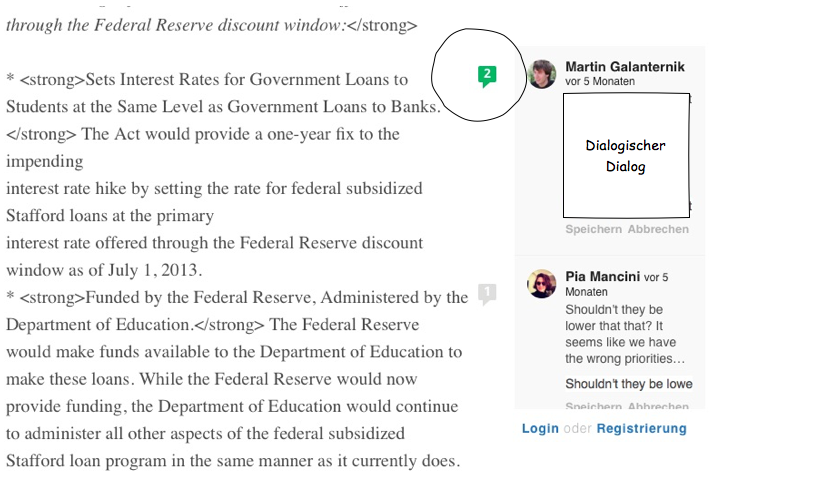
\includegraphics[width=1\textwidth]{img/democracyos.png}
\caption{Mögliche Anbindung der DSL an DemocracyOS}
\label{democracyos}
\end{figure}

DemocracyOS bietet die Möglichkeit Textpassagen eines Vorschlags zu kommentieren und dadurch einen parallelen Diskussionsstrang zu eröffnen. 
Hier könnte unsere \ac{DSL} eingebunden werden (vgl. \autoref{democracyos}, die Box \enquote{Dialogischer Dialog} kann  mit \autoref{faktencheck} gefüllt werden), um die Diskussion unterstützen.

Denkbar wäre auch, mit Blick auf quantifizierte Aussagen, dass Nutzer die Möglichkeit für Angriffe vorgeschlagen bekommen.
Eine allquantifizierte Aussage könnte mit dem Hinweis \enquote{Bringen Sie mindestens 1 Gegenbeispiel} versehen werden und so schon ein Angriffsmuster vorschlagen.
Ähnliches ist auch für andere Aussagetypen denkbar.
Dies würde zu einer \emph{interaktionsgesteuerten} Demokratie-Plattform führen.

Ein Benutzer müsste von der dialogischen Logik nicht viel verstehen, er müsste lediglich mit der Plattform interagieren und würde so unbemerkt einen dialogischen Dialog führen.
Natürlich könnten und müssten entsprechend ansprechende Oberflächen, die eventuell Teile der Grammatik als graphische Elemente ausdrücken, entwickelt werden.

\subsection{Faktencheck} % Simon#

\begin{figure}[H]
\centering
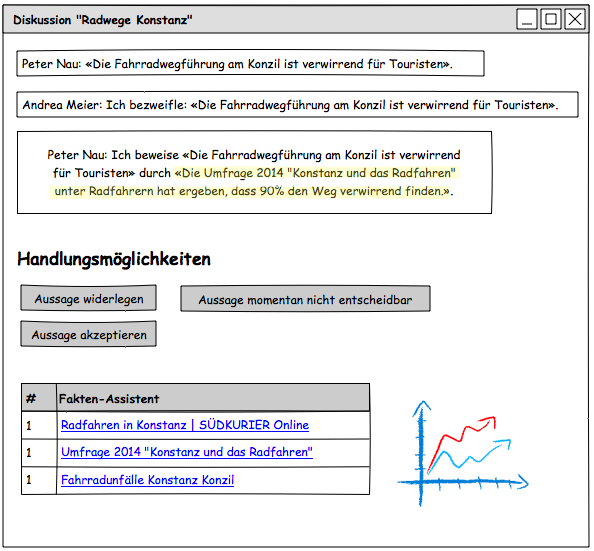
\includegraphics[width=1\textwidth]{img/faktencheck.png}
\caption{Faktencheck mit der DSL}
\label{faktencheck}
\end{figure}

Ein weiterer Einsatzzweck wäre ein (Echtzeit-)Faktencheck, der die partizipierenden Bürger bei der Wahrheitsfindung unterstützt.
Dieser Ansatz passt auch zur dialogischen Logik, welche hilft die \enquote{Wahrheit zu erarbeiten} (\cite{OrtnerDL}).

Eine Software könnte unter einem Dialog passend zu einer markierten Elementaraussage entsprechende Handlungsmöglichkeiten und intelligente Fakten präsentieren (vgl. \autoref{faktencheck}).
Dies hätte den Effekt eines \enquote{Intelligenzverstärkers}, der jedem Bürger das globale Wissen zur Seite stellt.

Auch die Anbindung von intelligenten Wissenssystemen (z. B. Watson \cite{Watson}), stellen interessante Möglichkeiten dar.
Durch das Aufbrechen eines komplexen Dialogs in kleine Elementaraussagen, können auch diese Systeme effektiver arbeiten und bessere Antworten liefern.
Insbesondere der Trend zu \emph{OpenData} könnte hier noch mehr Transparenz in Bürgerdiskussionen bringen.
Wird z. B. die Aussage getätigt, dass sich die Wasserqualität des Bodensees verschlechtert hat, könnten dank OpenData (und Smart Cities) sofort entsprechende Daten beim Fakten-Assistent (vgl. \autoref{faktencheck}) angezeigt werden, um diese Aussage im nächsten Schritt zu widerlegen oder zu bestätigen.

Wenn noch eine Ontologie mit den Begriffen der Diskussion angebunden wird (z. B. verwendete Begriffe im Raum Konstanz), dann könnte eine Art \emph{Stadt-Ontologie} erzeugt und Nutzern der Diskussionsplattformen geläufige Begriffe eingeblendet werden (z. B. anstatt Bus \enquote{Roter Arnold}).


\section{Politischer Unterrichtsdiskurs} % Tobi
Bei der Verwendung formaler oder auch dialogischer Logik liegt eine mathematische Betrachtung, bedingt durch die mathematische Natur der Logik, sehr nahe. 
Die dialogische Logik bildet im Projekt \textit{Logic} das logische Grundgerüst für den Dialog. Der Fokus liegt besonders auf dem Dialog in der Smart City, durch den der Bürger an politischen Dialogen und Diskussionen beteiligt werden soll.
Da die dialogische Logik in einem politischen Kontext betrachtet wird, unterscheidet sich das Projekt von bereits vorhandenen Projekten, wie beispielsweise das von Herrn Görz (\textit{Dialogische Logik und mathematischer Unterrichtsdiskurs}).
\textit{Logic} könnte im Umfeld des politischen Unterrichtsdiskurses zum Einsatz kommen, um politische Diskussionen zu analysieren, politische Aussagen kritisch zu hinterfragen und aktiv an politischen Diskussionen teilzunehmen und Schülern beziehungsweise Studierenden somit eine bestmögliche Lernerfahrung zu bieten.

% ============================ CHAPTER
\chapter{Fazit und Ausblick} % Tobi
Zusammenfassend kann festgestellt werden, dass es sich bei \textit{Logic} um einen ersten Versuch handelt, die dialogische Logik mit natürlicher Sprache in Verbindung zu bringen.
Dies ist besonders interessant im Kontext der Smart City, da dieses Thema, vor dem Hintergrund wachsender Urbanisierung, stetigem technischen Fortschritt und daraus resultierend einem Bedürfnis nach neuen Konzepten zur Beteiligung der Bürger, sehr zukunftsträchtig ist.

Aktuell ist \textit{Logic}  ein \textit{Proof of Concept}, wodurch gezeigt wurde, dass dialogische Logik prinzipiell auf diesem Gebiet eingesetzt werden kann und ein mächtiges Instrument zur gleichgestellten Beteiligung aller Bürger darstellt.
In aktuelle Projekte wie beispielsweise \textit{Liquid Democracy} wäre \textit{Logic} integrierbar, allerdings besteht in einigen Punkten noch Verbesserungspotential.
So beinhaltet das Projekt lediglich den syntaktischen Anteil, der semantische Anteil liegt jeweils im Umfang der Umsetzung des tatsächlichen Projekts. Daher ist der Aufwand bei der Entwicklung und Wartung größer als bei aktuellen Systemen. Dieser ergibt sich auch aus dem Einsatz von Tools der modellgetriebenen Softwareentwicklung.
Des Weiteren bestehen noch gewisse Einschränkungen bei den Formulierungen der Aussagen, da natürliche Sprache nicht ohne weiteres von Maschinen verstanden werden kann. Hierbei ist besonders die konkrete Syntax, die die Schnittstelle zum Benutzer darstellt, zu nennen. Dieser kommt eine besondere Rolle zu und bedarf, je nach Möglichkeit des maschinellen Verständnisses natürlicher Sprache, noch einem gewissen Weiterentwicklungsaufwand. Der Fokus liegt dabei auf einer möglichst geringen Einschränkung erlaubter Formulierungen, um die Benutzung durch den Bürger so einfach wie möglich zu gestalten.

Diese Einschränkung könnte durch den Einsatz eines Systems wie \textit{Watson} von IBM deutlich verringert werden, da dieses die Qualität beim Verständnis natürlicher Sprache deutlich erhöhen würde und somit die Freiheiten bei den erlaubten Formulierungen deutlich steigern würde. Zudem würde sich mittels eines solchen Systems das weite Feld der Verwendung gesprochener Aussagen öffnen.
Systeme, die auf der Grundlage der dialogischen Logik aufbauen, haben das Potential als Bindeglied zwischen digitaler Beteiligung und deren technischen Hürden auf der einen Seite und der breiten Masse der Bürger ohne speziellen technischen Bildungshintergrund auf der anderen Seite zu fungieren. Diese könnten als eine Art Katalysator der Demokratie 2.0 dienen, denn neue Formen des Zusammenlebens erfordern neue Formen der Beteiligung. Hierbei stellen Systeme wie \textit{Logic}, mit ihren aktuell noch etwas starken Einschränkungen, nur einen ersten Schritt dar. Das Ziel ist hierbei eine nahtlose Integration der dialogischen Logik als Grundlage aller Dialoge und Diskussionen.
Dies würde zu einer Steigerung der Effizienz bereits vorhandener Systeme beitragen und deren Akzeptanz deutlich erhöhen.
Zudem könnte so der Generation-Gap zwischen Digital Natives und älteren Mitbürgern möglichst stark verringert, wenn nicht sogar beseitigt werden.

In Zeiten voranschreitender Politikverdrossenheit stellt diese Art von Systemen eine besondere Chance dar, das Interesse an (politischer) Beteiligung durch Beseitigung von Hürden wieder spürbar zu steigern. Dialoge könnten von parteiorientierten Entscheidungen, wie sie bei Wahlen vorzufinden sind, losgelöst werden und sich hin zu einer Orientierung an einzelnen Themen entwickeln. Dadurch würde sich Bürgern ein erweitertes Spektrum der Beteiligung auf allen Ebenen öffnen.
Die daraus resultierende Dynamik könnten genutzt werden, um dem politischen Bürger zu neuer Blüte zu verhelfen und die aktive Gestaltung der Zukunft wieder in den Fokus eines jeden Einzelnen zu rücken.
 
% ============================ ENDE HAUPTTEIL







% ============================ LITERATURVERZEICHNIS
\begin{singlespace}
\begin{thebibliography}{9}

% SORT BY AUTHOR LASTNAME

\bibitem[Ecl12]{Spray}
  Eclipse Labs,
  \emph{spray - A quick way of creating Graphiti},
  \url{https://code.google.com/a/eclipselabs.org/p/spray/},
  besucht am 18.06.2015.   
  
\bibitem[IBM15]{Watson}
  IBM Deutschland GmbH
  \emph{IBM Watson},
  \url{http://www-05.ibm.com/de/watson/},
  besucht am 18.06.2015.
  
\bibitem[Kes15]{GitHubCode}
  Simon Kessler, Tobias Keh,
  \emph{Dialogische Logik DSL Quellcode},
  \url{https://github.com/sikessle/dialogical-logic-dsl},
  besucht am 20.06.2015.

\bibitem[Ort15]{OrtnerDL}
  Prof. Dr. Erich Ortner,
  \emph{Einf{\"u}hrung in die Dialogische Informatik},
  HTWG Präsentation,
  2015.
  
\bibitem[Dem15]{DemocracyOS}
  The DemocracyOS Foundation,
  \emph{DemocracyOS - Power in your hands},
  \url{http://democracyos.org},
  besucht am 25.06.2015.
  
\bibitem[Ecl15a]{Ecore}
  The Eclipse Foundation,
  \emph{Eclipse Modeling Framework (EMF)},
  \url{https://eclipse.org/modeling/emf/},
  besucht am 26.06.2015.

\bibitem[Ecl15b]{Xtext}
  The Eclipse Foundation,
  \emph{Xtext - Language Development Made Easy!},
  \url{https://eclipse.org/Xtext/},
  besucht am 25.06.2015.
  
\bibitem[Ecl15c]{XtextLoadJava}
  The Eclipse Foundation,
  \emph{Xtext FAQ - How do I load my model in a standalone Java application?},
  \url{http://wiki.eclipse.org/Xtext/FAQ#How_do_I_load_my_model_in_a_standalone_Java_application.C2.A0.3F},
  besucht am 25.06.2015.
  
  

\end{thebibliography}
\end{singlespace}
% ============================ ENDE LITERATURVERZEICHNIS



\end{document}

